\documentclass[journal]{IEEEtran}

\usepackage{algorithm}
\usepackage{algorithmicx}
\usepackage{algpseudocode}
\usepackage{amssymb}
\usepackage{graphicx}
\usepackage{setspace}
\usepackage{color}
\usepackage{amsmath,amssymb,amsfonts,amsthm}
\usepackage{bm}
\usepackage{multirow}
\usepackage{subfig}
\usepackage{tabularx}
\usepackage{amsfonts}
\usepackage{comment}
\usepackage{slashbox}
\usepackage{rotating}
\usepackage{booktabs,threeparttable}
\renewcommand*{\thefootnote}{\fnsymbol{footnote}}
\usepackage{pdfpages}

\begin{document}
\title{Thesis during summer vacation}


% author names and affiliations
% use a multiple column layout for up to three different
% affiliations
\author{Yin-Hong Hsu}

% make the title area
\maketitle
% in the abstract
% \begin{abstract}
% 	To briefly describe what I have done in this semester.
% 	The each subjects are list as a section. And in each subject, all topics are listed.      
% \end{abstract}

% no keywords




% For peer review papers, you can put extra information on the cover
% page as needed:
% \ifCLASSOPTIONpeerreview
% \begin{center} \bfseries EDICS Category: 3-BBND \end{center}
% \fi
%
% For peerreview papers, this IEEEtran command inserts a page break and
% creates the second title. It will be ignored for other modes.
\IEEEpeerreviewmaketitle
\section{Priority-Based Random Access... ~\cite{Zangar16}}
\begin{itemize}
    \item {Seperating device into several priority level according to their delay sensitivity} 
    \item {Send msg3 with a overload indicator which means the retry times}
    \item {There have two variable P1 and P2 as drop rate of group 1 and group2 to cope the QoS requirement}
\end{itemize}
\section{Priority-Based Random Access... ~\cite{Guan16}}
\begin{itemize}
    \item {They also seperate device into high, medium, low priority level} 
    \item {To adjust system parameter dynamically to cope different situation}
    \item {Estimate conjestion level by the number of collision preamble instead of retry times of device}
    \item \textbf{In NB-IoT, there is not QoS concept. So it is not necessary to have different priority level}
\end{itemize}
\section{D2D-Based Grouped Random Access... ~\cite{HanHSDS17}}
\begin{itemize}
    \item {Seperating device into device classes} 
    \item {Reducing the times of random access by make several device into a group}
    \item {Classify device by device class and geolocation information}
\end{itemize}
\section{Optimal Resource Dedication... ~\cite{HanHS17}}
\begin{itemize}
    \item {Seperating device into device classes} 
    \item {Discussing the way to allocate radio network resource}
    \item {Purposed an algorithm to dedicate radio network resource to each special device class}
\end{itemize}
\section{Future Work}
\begin{itemize}
	\item {Random Access on NB-IoT study }
	\item {NB-IoT in OAI study ~\cite{OAI}}
\end{itemize}
% \section{Work on Retransmission-Based Access Control ...}
\label{Retransmission-Based}
    \begin{itemize}
        \item {Revise the paper format}
        \item {To reproduce the simulation proposed in the paper}
        \item {Compare the simulation result with others}
        \begin{itemize}    
            \item[-]{DACB by Suyang Duan}
            \item[-]{TRAO by German Corrales Madueno}
            \item[-]{...}
        \end{itemize}
        \item {To survey for the different on access barring mean between NB-IoT and LTE}  Fig.~\ref{fig_Access_Barring}
        \item {To study for the process and detail of the access control technology (EAB)}
    \end{itemize}
    
% \section{Wearable Project}
\label{project}
    An Android project to communicate with two BLE device, the bracelet and glass.
    The bracelet can be distinct the color of an object, alarm when it's close to other objects.
    The glasses can read the QRcode Message and know it's in a crowded place.
    This application can send/receive message to/from device, and speak the message from device to user.
    \begin{itemize}
        \item {New UI flow} Fig.~\ref{fig_UI_flow}
        \item {Bracelet device}
        \begin{itemize}    
            \item[-]{Seek Bracelet - change the notification way to the alarm instead of vibrate}
            \item[-]{Color Detection - new data format}
            \item[-]{Distance Detection - the bracelet only work well once}
            \item[-]{Power Information - hard code in bracelet}
            \item[-]{Connection switch - new connect and disconnect approach in new design}
        \end{itemize}
        \item {New layout, and new layout...} Fig.~\ref{fig_UI_design}
        \item {To demonstrate the application successfully  on the final exhibition}
    \end{itemize}
    
    

% \section{Work on Design of Region-based ...}
\label{Retransmission-Based}
    \begin{itemize}
        \item {Read paper to know the background knowledge}
        \item {To implement the experiment for 4 functions mentioned in paper}
        \begin{itemize}    
            \item[-]{Setup}
            \item[-]{Key Generation}
            \item[-]{Signing}
            \item[-]{Verification}
        \end{itemize}
        A project on Android, to run four functions listed above individually and show their CPU usage and time consumption.
    \end{itemize}

	% \begin{figure}[t]
 %    \centering
 %    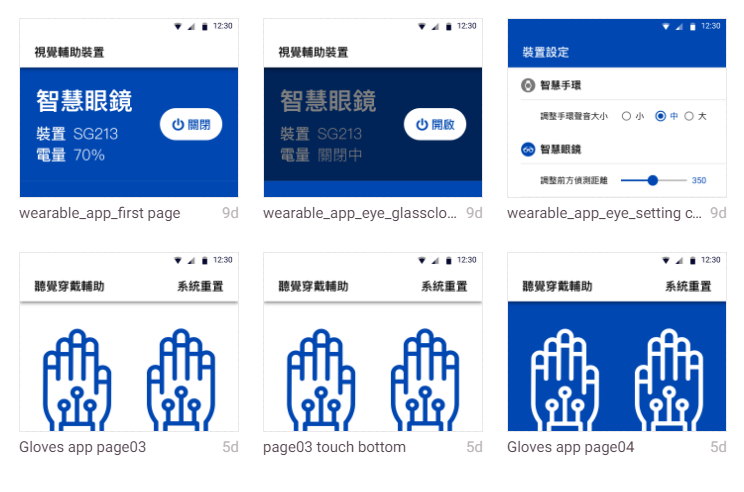
\includegraphics[width=3.5in]{figure/layout.png}
 %    \caption{They change the UI for several times}
 %    \label{fig_UI_flow}
 %    \end{figure}
 %    \begin{figure}[t]
 %    \centering
 %    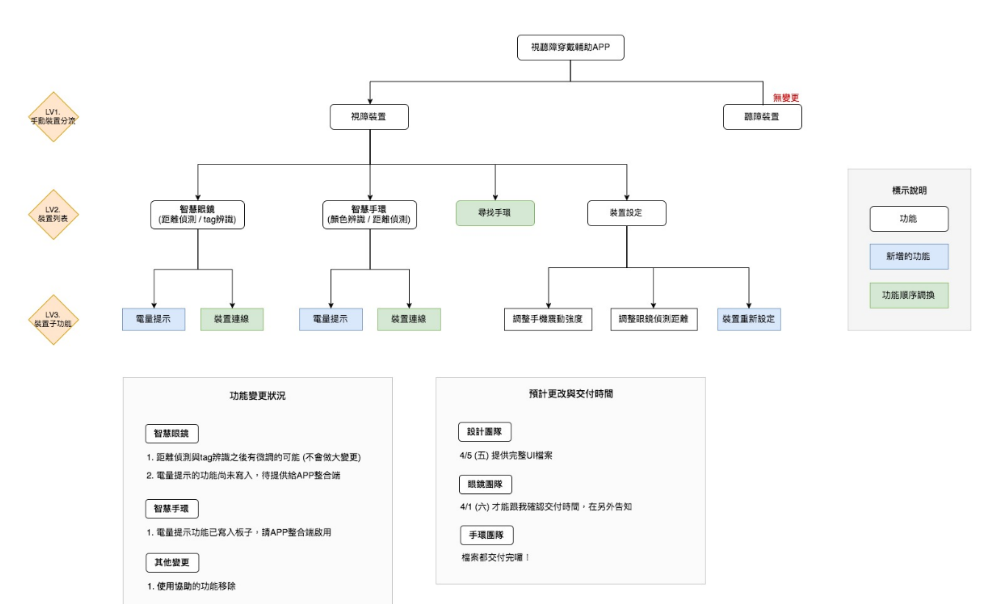
\includegraphics[width=3.5in]{figure/uiflow.png}
 %    \caption{New Design for User Interface} 
 %    \label{fig_UI_design}
 %    \end{figure}
 %    \begin{figure}[t]
 %    \centering
 %    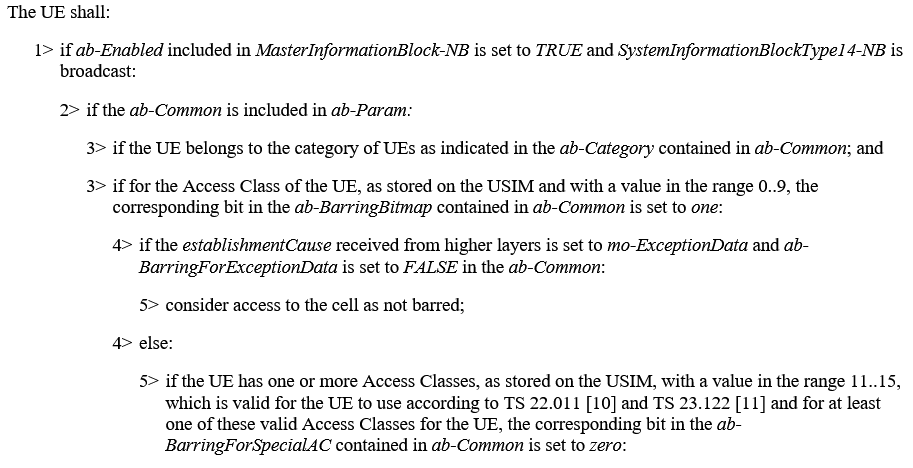
\includegraphics[width=3.5in]{figure/ab.png}
 %    \caption{The access barring process for NB-IoT}
 %    \label{fig_Access_Barring}
 %    \end{figure}

% conference papers do not normally have an appendix

\bibliographystyle{ieeetran}  % 使用 IEEE Trans 期刊格式
{\footnotesize
\bibliography{IEEEabrv,my_bib}  %reference 所需的bib檔
}


% that's all folks
\end{document}


